\documentclass[11pt]{article}
\usepackage[margin=2.5cm]{geometry}
\usepackage[utf8]{inputenc}
\usepackage[spanish]{babel}
\usepackage{graphicx}
\usepackage{amsmath}
\usepackage{amssymb}
\usepackage{booktabs}
\usepackage{hyperref}
\usepackage{float}
\usepackage{tikz}
\usepackage{verbatim}
\usepackage{xcolor}
\usetikzlibrary{arrows.meta, positioning, calc}

\hypersetup{
  colorlinks=true,
  linkcolor=black,
  citecolor=black,
  urlcolor=blue,
  pdftitle={Gemelo digital del beamline -- Reporte tecnico},
  pdfauthor={Taller MIT-UNAL}
}

\title{\Large Gemelo digital del beamline\\[0.3em]
  \large Reporte técnico del proyecto}
\author{Taller MIT--UNAL, Medellín}
\date{Julio de 2026}

\begin{document}
\maketitle

\begin{abstract}
\noindent
Este documento describe, de punta a punta, el gemelo digital de un beamline
de iones desarrollado sobre SIMION~8.1 para el taller MIT--UNAL. El sistema
aprende un modelo surrogate (un \emph{hurdle model}: clasificador de señal +
proceso gaussiano físico) a partir de un presupuesto fijo de 100 evaluaciones
reales, lo valida contra 394 puntos reales nunca usados en el entrenamiento,
y lo usa para resolver dos tareas de control --maximizar la transmisión de
iones y alcanzar una consigna objetivo-- sin necesitar SIMION en el momento
de predecir. El documento cubre tanto la metodología científica (qué se
modela, cómo, y con qué evidencia empírica se tomó cada decisión de diseño)
como la arquitectura del repositorio de software que la implementa, de modo
que sirva como referencia única para entender y reproducir el proyecto
completo. Para el informe original entregado en el taller, organizado según
las 7 secciones de la rúbrica, ver \texttt{report/informe.pdf}.
\end{abstract}

\tableofcontents

% =============================================================================
\section{Introducción y contexto}
% =============================================================================

El reto consiste en dirigir un haz de 500 iones $^{28}$Si$^+$ (15\,eV) a
través de una pila de electrodos electrostáticos hasta un detector, usando
SIMION~8.1 como simulador de trayectorias. Ocho electrodos son controlables
(lentes Einzel, curvador cuadrupolar y placas deflectoras); el resto quedan
fijos (fuente de alto voltaje, detector, tierras). Correr SIMION es costoso
--cada evaluación es una simulación completa de trayectorias-- así que el
taller impone un \textbf{presupuesto de entrenamiento de 100 evaluaciones
reales} para construir un modelo surrogate (el ``gemelo digital'') capaz de:

\begin{enumerate}
  \item \textbf{Predecir} la transmisión (iones que llegan al detector) para
  cualquier combinación de voltajes, con incertidumbre honesta.
  \item \textbf{Resolver dos tareas de control} apoyándose solo en el gemelo:
  encontrar los voltajes que maximizan la transmisión esperada
  (\emph{dirección}), y encontrar los voltajes que producen una transmisión
  objetivo dada (\emph{consigna inversa}).
  \item \textbf{Verificarse} contra corridas reales de SIMION, tanto en
  predicción puntual como en las recomendaciones de control.
\end{enumerate}

Antes de este proyecto ya existía un historial de \textbf{824 evaluaciones
reales} generadas por búsqueda bayesiana (Optuna) sobre SIMION
(\texttt{simulation/optimizer.py}). La estrategia central de este trabajo fue
\textbf{no desperdiciar ese historial}: en vez de gastar el presupuesto de
100 evaluaciones en puntos nuevos elegidos a ciegas, se seleccionaron 100
puntos de ese historial ya existente por muestreo estratificado, dejando el
resto (${\sim}394$ puntos) como conjunto de validación real y gratuito --algo
mucho más informativo que cualquier separación sintética.

% =============================================================================
\section{Arquitectura del repositorio}
% =============================================================================

El repositorio separa datos, simulación, código del modelo e informes en
carpetas independientes, para que cada pieza pueda evolucionar (y
versionarse) por separado:

\begin{verbatim}
.
+-- src/digital_twin/     El gemelo digital: modelo, control y experimentos.
|   +-- real_data.py          Carga y particion train/test (datos reales).
|   +-- gp_model.py           Hurdle model (clasificador + GP fisico).
|   +-- control.py            Tareas de direccion y consigna inversa.
|   +-- simion_interface.py   Conexion a SIMION real.
|   +-- data_collection.py    Utilidades de recoleccion (active learning).
|   +-- main.py               Pipeline completo, de punta a punta.
|   +-- kernel_experiment.py  Comparacion de kernels del regresor.
|   +-- retrain_experiment.py Efecto de agregar mas sondas al training.
|   +-- gradient_eps_study.py Estudio del paso eps del gradiente.
|   +-- gradient_retrain_check.py  Chequeo held-out del gradiente.
|   +-- verify_v2.py          Verificacion real de las tareas de control.
|   +-- prototype_synthetic/  Simuladores sinteticos de la etapa de diseno
|                              (no forman parte del gemelo entregado).
+-- data/                 Datos reales de SIMION y caches de reproducibilidad.
|   +-- beamline_results.csv      824 corridas reales (Optuna + SIMION).
|   +-- beamline_study.db         Estudio de Optuna que las genero.
|   +-- gradient_probe_cache.npz      16 sondas de densificacion (congeladas).
|   +-- gradient_eps_study_cache.npz  Estudio de paso eps (congelado).
+-- simulation/           Simulacion SIMION (geometria, .iob) y el optimizador.
|   +-- optimizer.py              Script Optuna + SIMION original.
|   +-- SimpleSetUp.iob / .fly2   Definicion del vuelo de iones.
|   +-- electrode_*.stl, electrode_.PA#   Geometria de electrodos.
+-- report/               Informes (LaTeX + PDF) y generador de figuras.
    +-- informe.tex / .pdf          Informe original (rubrica del taller).
    +-- reporte_tecnico.tex / .pdf  Este documento.
    +-- generate_figures.py         Regenera las figuras desde datos reales.
\end{verbatim}

La Figura~\ref{fig:pipeline} resume el flujo de datos de punta a punta.

\begin{figure}[H]
\centering
\begin{tikzpicture}[
  node distance=1.1cm and 1.6cm,
  box/.style={draw, rounded corners, align=center, minimum height=1.1cm,
              minimum width=3.2cm, font=\small},
  arr/.style={-{Stealth[length=2.2mm]}, thick}
]
  \node[box] (data)   {\texttt{data/}\\[2pt] 824 corridas reales};
  \node[box, right=of data] (split) {\texttt{real\_data.py}\\[2pt] partición
    estratificada\\ 100 train / 394 test};
  \node[box, right=of split] (model) {\texttt{gp\_model.py}\\[2pt] hurdle model\\
    (clasificador + GP)};
  \node[box, below=of model] (control) {\texttt{control.py}\\[2pt] dirección /
    consigna\\ (región de confianza)};
  \node[box, left=of control] (verify) {\texttt{simion\_interface.py}\\[2pt]
    verificación real};
  \node[box, left=of verify] (report) {\texttt{report/}\\[2pt] figuras e
    informes};

  \draw[arr] (data) -- (split);
  \draw[arr] (split) -- (model);
  \draw[arr] (model) -- (control);
  \draw[arr] (control) -- (verify);
  \draw[arr] (verify) -- (report);
  \draw[arr] (model.south) |- ($(report.north)+(0,0.55)$) -- (report.north);
\end{tikzpicture}
\caption{Flujo del pipeline: de los datos reales congelados en \texttt{data/}
hasta los informes en \texttt{report/}, pasando por el ajuste del modelo y las
tareas de control. Las flechas de vuelta representan la verificación real
(SIMION) y la generación de figuras.}
\label{fig:pipeline}
\end{figure}

\subsection{Reproducibilidad}

\begin{verbatim}
pip install -r requirements.txt
cd src/digital_twin
python main.py
\end{verbatim}
Con las semillas fijas (\texttt{SEED=42}) y los cachés de \texttt{data/}
incluidos, esto reproduce exactamente los números de este reporte sin
necesitar una instalación local de SIMION. Verificar recomendaciones de
control contra SIMION real, o regenerar los cachés de densificación, sí
requiere SIMION~8.1 instalado (ver \texttt{README.md}).

% =============================================================================
\section{Datos: recolección y partición}
% =============================================================================

De las 824 corridas de \texttt{optimizer.py}, 330 fallaron con un error de
subproceso. La causa identificada fue interferencia de sincronización de
OneDrive sobre el archivo de campo \texttt{electrode\_.PA0} (reescrito en
cada evaluación); tras excluir la carpeta de la sincronización, la tasa de
error cayó a prácticamente cero. Quedaron \textbf{494 evaluaciones reales
válidas}: 130 con señal (transmisión $>0$) y 364 en cero (zona muerta, 74\,\%
de los puntos).

Del presupuesto de 100 evaluaciones, se eligieron 100 de esos 494 puntos ya
existentes mediante \emph{farthest-point sampling} (muestreo de máxima
distancia mínima) aplicado por separado a la región de señal y a la zona
muerta --45 y 55 puntos respectivamente-- para que el pico de transmisión
quedara bien representado aunque sea la minoría de los datos. Los 394 puntos
restantes, nunca usados para entrenar, forman el conjunto de validación real
(Figura~\ref{fig:cobertura}).

\begin{figure}[H]
  \centering
  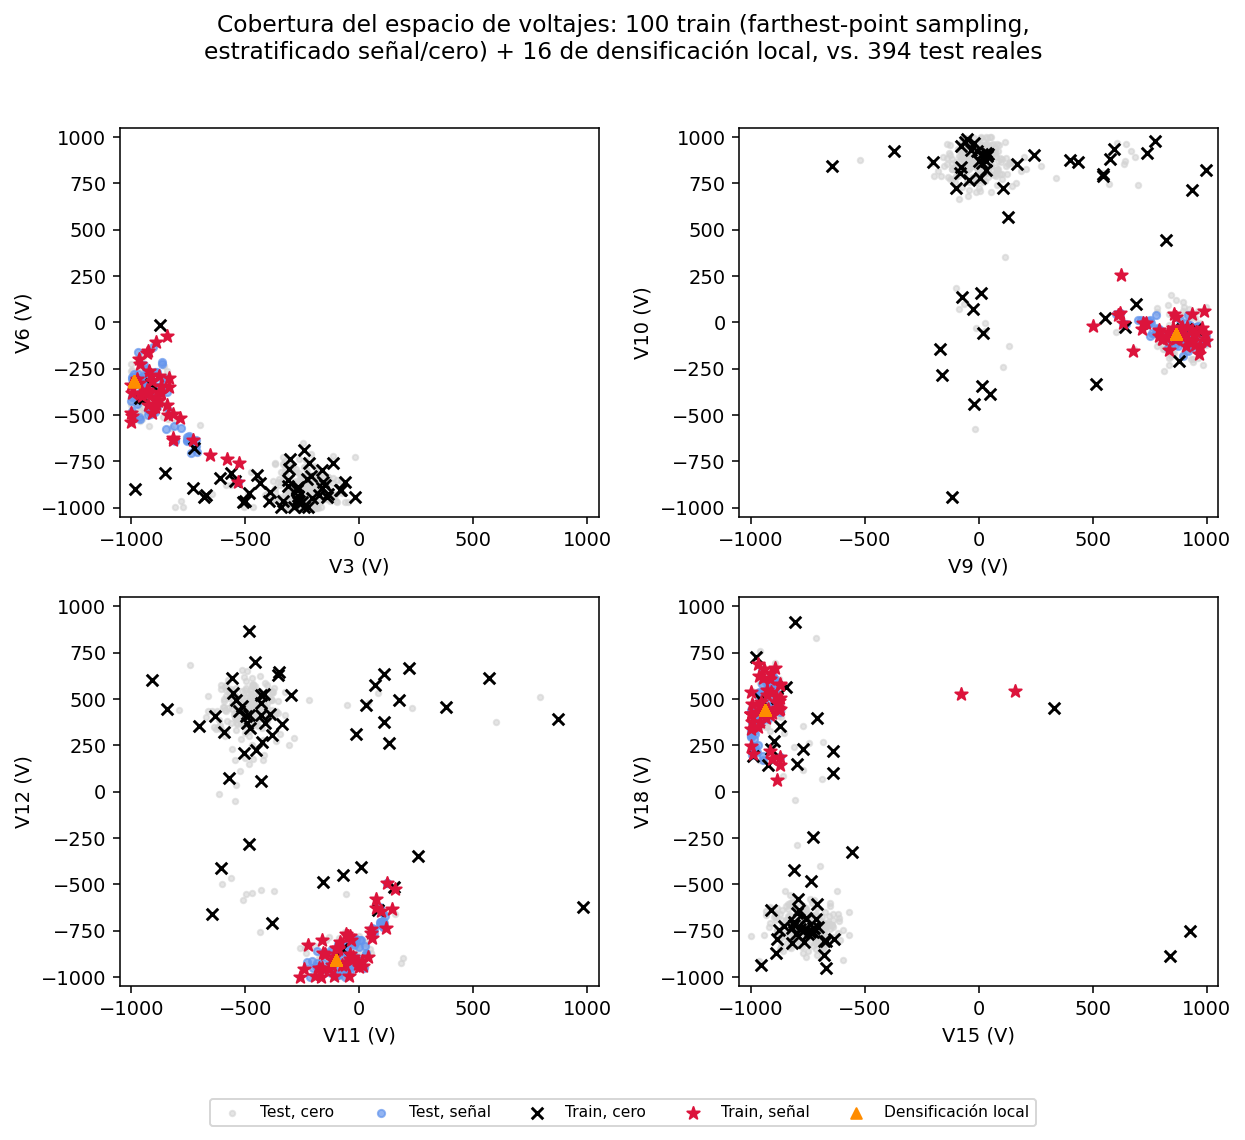
\includegraphics[width=0.95\textwidth]{figures/fig1_cobertura.png}
  \caption{Cobertura del espacio de voltajes en cuatro proyecciones 2D. Los
  100 puntos de entrenamiento (cruces y estrellas) se distribuyen por todo el
  rango explorado, no solo cerca del pico. Los triángulos naranjas son los 16
  puntos de densificación local (Sección~\ref{sec:diferenciabilidad}).}
  \label{fig:cobertura}
\end{figure}

Adicionalmente se densificó localmente con 16 puntos reales alrededor del
mejor voltaje conocido, cada uno promediado sobre 5 corridas reales de SIMION
por el ruido intrínseco de la fuente de iones (Sección~\ref{sec:limitaciones}).
En total: \textbf{100 + 16 = 116 puntos de entrenamiento}, usando 180
llamadas reales a SIMION en total ($100 + 16\times5$).

% =============================================================================
\section{Metodología del modelo}
% =============================================================================

\subsection{Arquitectura: hurdle model}

Con el 74\,\% de los puntos válidos en cero, un solo proceso gaussiano
ajustando toda la transmisión de una vez predice cerca de cero en todas
partes. El problema se separa en dos etapas (\emph{hurdle model},
implementado en \texttt{gp\_model.BeamlineTwin}):

\begin{itemize}
  \item \textbf{Etapa A -- clasificador}: un \texttt{GaussianProcessClassifier}
  (kernel RBF con un length-scale por dimensión, ARD) entrenado con los 116
  puntos completos, predice $P(\text{señal}\mid V)$.
  \item \textbf{Etapa B -- regresor de magnitud}: un GP (kernel
  $\text{ConstantKernel}\times\text{Matérn}_{\nu=1.5}\text{(ARD)} +
  \text{WhiteKernel}$, con \texttt{log1p} en la salida y \texttt{StandardScaler}
  en entradas y salida) entrenado \textbf{solo} con los puntos de señal.
\end{itemize}

Ambas etapas reciben 10 features de entrada: los 8 voltajes más $V_3^2$ y
$V_6^2$ (Sección~\ref{sec:fisica}).

\subsection{Feature física: ley $V^2$ de la lente Einzel}
\label{sec:fisica}

Los electrodos $V_3$ y $V_6$ son lentes Einzel; su potencia de enfoque
escala como $(V_{\text{lente}}/V_{\text{haz}})^2$ (fórmula de lente delgada
electrostática), independiente del signo del voltaje. Se agregan $V_3^2$ y
$V_6^2$ como entradas adicionales para que el GP tenga esa cantidad
disponible explícitamente, sin depender de que el kernel la infiera solo de
datos escasos.

\subsection{Selección de kernel}

Se comparó el kernel del regresor de magnitud contra el mismo test real de
394 puntos (\texttt{kernel\_experiment.py}), sin llamadas nuevas a SIMION:

\begin{center}
\begin{tabular}{lcc}
\toprule
Kernel & $R^2$ región informativa & MAE (iones) \\
\midrule
RBF                & 0.203 & 9.04 \\
Matérn $\nu=1.5$ (elegido) & \textbf{0.237} & 9.01 \\
Matérn $\nu=2.5$   & 0.232 & 9.00 \\
\bottomrule
\end{tabular}
\end{center}

Matérn $\nu=1.5$ asume una función menos suave que RBF, consistente con un
pico de transmisión angosto y una respuesta física que no es infinitamente
diferenciable.

\subsection{Combinando las dos etapas}

Con $T = Z\cdot M$, $Z\sim\text{Bernoulli}(p)$ y $M$ la magnitud (media
$\mu_B$, varianza $\sigma_B^2$), la ley de varianza total da:
\begin{equation}
  \mathbb{E}[T] = p\,\mu_B, \qquad
  \text{Var}[T] = p(1-p)\,\mu_B^2 + p\,\sigma_B^2 .
\end{equation}
Esto es exactamente lo que implementa \texttt{BeamlineTwin.predict\_combined()}.
El primer término de la varianza crece cuando el clasificador no sabe si hay
señal; el segundo, cuando el regresor no sabe cuánta. Ambas salidas se
recortan a $[0,500]$.

% =============================================================================
\section{Validación}
% =============================================================================

Sobre los 394 puntos de test reales (nunca vistos en entrenamiento):

\begin{center}
\begin{tabular}{lcc}
\toprule
Métrica & Global (394 pts) & Región informativa (85 pts con señal) \\
\midrule
$R^2$ & 0.161 & \textbf{0.237} \\
MAE (iones) & 6.81 & 9.01 \\
\bottomrule
\end{tabular}
\end{center}

El clasificador (Etapa A) obtiene \emph{accuracy}$=0.845$,
\emph{precision}$=0.582$ y \textbf{recall}$=1.000$: nunca descarta un punto
que en realidad tiene señal, a cambio de marcar de más algunos puntos en
cero como posible señal -- el error preferible, dado que perderse la región
de señal es mucho más costoso (Figura~\ref{fig:predicho}).

\begin{figure}[H]
  \centering
  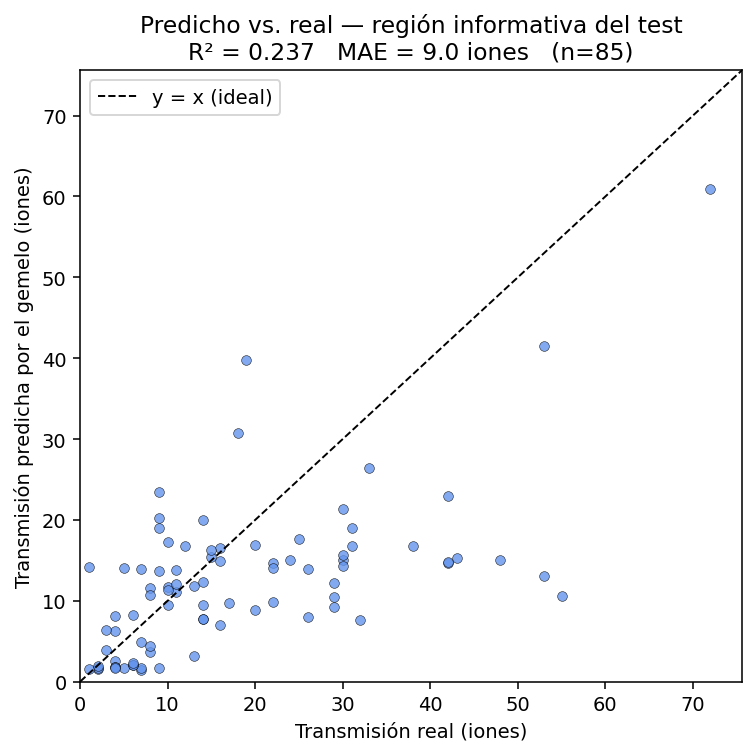
\includegraphics[width=0.6\textwidth]{figures/fig2_predicho_vs_real.png}
  \caption{Transmisión predicha vs.\ real, solo en los 85 puntos de test con
  señal.}
  \label{fig:predicho}
\end{figure}

La desviación estándar combinada (Figura~\ref{fig:honestidad}) es más alta
justo donde el clasificador está indeciso ($P(\text{señal})\in[0.4,0.6]$) y
más baja donde está seguro -- el comportamiento esperado de una
incertidumbre honesta.

\begin{figure}[H]
  \centering
  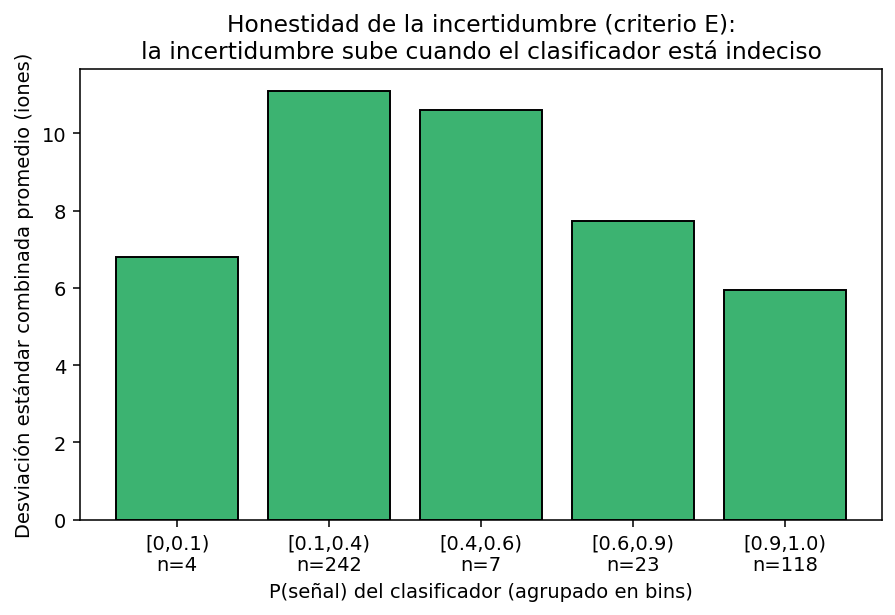
\includegraphics[width=0.6\textwidth]{figures/fig3_honestidad_incertidumbre.png}
  \caption{La incertidumbre combinada crece cuando el clasificador está
  indeciso.}
  \label{fig:honestidad}
\end{figure}

\subsection{¿Vale la pena agregar más sondas al entrenamiento?}
\label{sec:validacion-retrain}

Se probó reentrenar agregando las 32 sondas adicionales del estudio de
gradiente (Sección~\ref{sec:diferenciabilidad}, $\varepsilon=5$ y
$\varepsilon=10$\,V) al modelo base de 116 puntos
(\texttt{retrain\_experiment.py}):

\begin{center}
\begin{tabular}{lcc}
\toprule
Puntos de entrenamiento & $R^2$ región informativa & MAE (iones) \\
\midrule
116 (modelo entregado) & \textbf{0.237} & 9.01 \\
148 (+32 sondas de gradiente) & 0.228 & 9.12 \\
\bottomrule
\end{tabular}
\end{center}

Agregar esas 32 sondas \textbf{degrada} el ajuste global: están apiñadas
alrededor de un único punto ancla y desequilibran el GP en el resto del
espacio. Por eso el modelo entregado se queda en 116 puntos.\footnote{El
informe original (\texttt{informe.pdf}) reporta una caída mayor, a
$R^2=-0.07$, para este mismo experimento. Al reproducir
\texttt{retrain\_experiment.py} con las versiones de \texttt{scikit-learn}
fijadas en \texttt{requirements.txt} se obtiene $R^2=0.228$: la dirección de
la conclusión (agregar esas sondas degrada el ajuste global) se mantiene,
pero la magnitud exacta es sensible a la versión de la librería usada para
reoptimizar los hiperparámetros del kernel. Los números de esta sección son
los reproducibles con el entorno fijado en este repositorio.}

% =============================================================================
\section{Control}
% =============================================================================

\subsection{El problema: optimizar libremente sobre el gemelo es peligroso}

Optimizar \texttt{predict\_combined} sin restricciones sobre todo
$\pm1000\,$V encuentra voltajes donde el modelo está \emph{confiadamente
equivocado}: verificado con SIMION real, una recomendación con predicción
${\sim}35$ iones dio \textbf{0 iones reales}. Ni penalizar la incertidumbre
en el objetivo (\emph{lower confidence bound}) lo arregla -- el modelo tiene
std bajo justo donde falla. Con solo 45--61 puntos de señal en 8 dimensiones,
el pico real es más angosto de lo que el GP puede resolver.

\subsection{La solución: radio de confianza calibrado con SIMION real}

Ambas tareas de control (\texttt{control.py}) restringen la búsqueda
(\texttt{scipy.optimize.minimize}, L-BFGS-B) a una caja alrededor de un
\textbf{punto real observado}, con un radio calibrado corriendo SIMION real a
distintos valores:

\begin{center}
\begin{tabular}{lcccccc}
\toprule
Radio (V) & 150 & 40 & 20 & 15 & 10 & 5 \\
\midrule
Transmisión real (iones) & 1 & 0 & 18 & 31 & 29 & \textbf{39} \\
\bottomrule
\end{tabular}
\end{center}

Se fijó \textbf{radio $=5\,$V}. La caja de \emph{dirección} se centra en el
mejor voltaje real conocido (72 iones); la de \emph{consigna inversa} se
centra en el punto real cuya transmisión observada está más cerca del
objetivo, no en el pico -- anclar en el pico obligaba al gemelo a modelar la
ladera descendente de la campana y dio un error real de 13.8 iones en una
versión anterior.

\subsection{Resultado final verificado}

Cada número real es el promedio de 5 corridas reales de SIMION:

\begin{center}
\begin{tabular}{lccp{4.6cm}}
\toprule
Tarea & Predicho por el gemelo & Real (SIMION, prom.\ 5) & Resultado \\
\midrule
Dirección (max.)     & 63.3 & $55.2\pm6.4$ & $C=0.767$ (77\,\% del óptimo real, 72 iones) \\
Consigna (obj.\ =35) & 29.9 & $36.8\pm5.0$ & error $=1.8$ iones ($<$ ruido de la máquina) \\
\bottomrule
\end{tabular}
\end{center}

\begin{figure}[H]
  \centering
  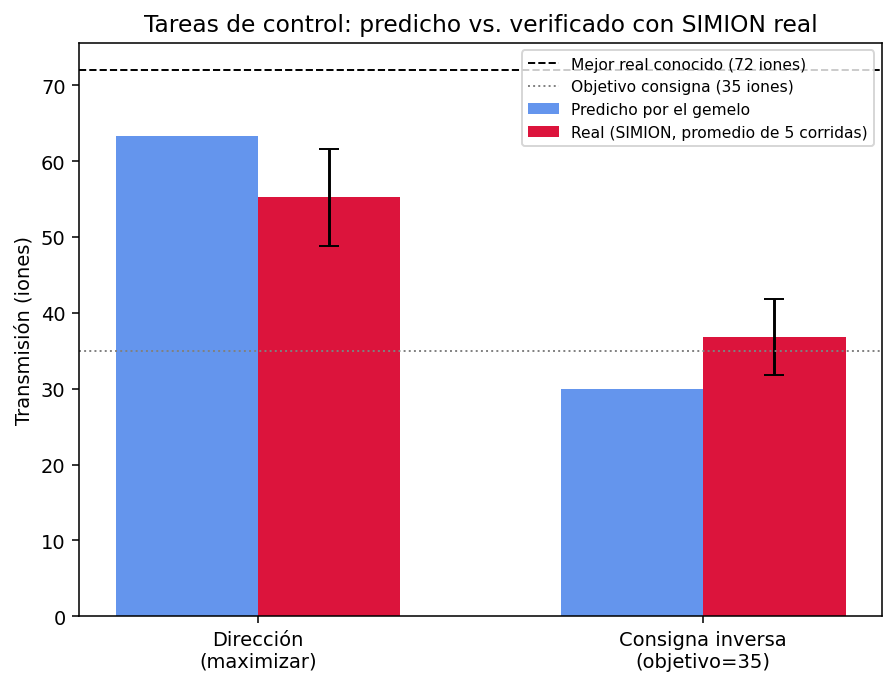
\includegraphics[width=0.6\textwidth]{figures/fig4_control.png}
  \caption{Resultados de control: predicho por el gemelo vs.\ verificado con
  SIMION real.}
  \label{fig:control}
\end{figure}

Las funciones \texttt{verify\_with\_simion()} y
\texttt{verify\_gradient\_with\_simion()} (\texttt{control.py}) ejecutan estas
verificaciones; no se invocan automáticamente desde \texttt{main.py} porque
consumen evaluaciones reales adicionales (fuera del presupuesto de
entrenamiento, pero reales al fin).

% =============================================================================
\section{Diferenciabilidad}
\label{sec:diferenciabilidad}
% =============================================================================

\subsection{Antes y después de la densificación local}

Se comparó el gradiente del gemelo contra diferencias finitas de SIMION real
($\varepsilon=1\,$V) en el punto ancla. Antes de densificar (solo 100 puntos
base), la similitud coseno entre ambos gradientes era $-0.612$ --¡apuntaban
casi en dirección opuesta! Después de densificar con los 16 puntos reales
locales, subió a $-0.049$: ya no contradice la realidad, aunque tampoco
concuerda bien todavía (Figura~\ref{fig:gradiente}).

\begin{figure}[H]
  \centering
  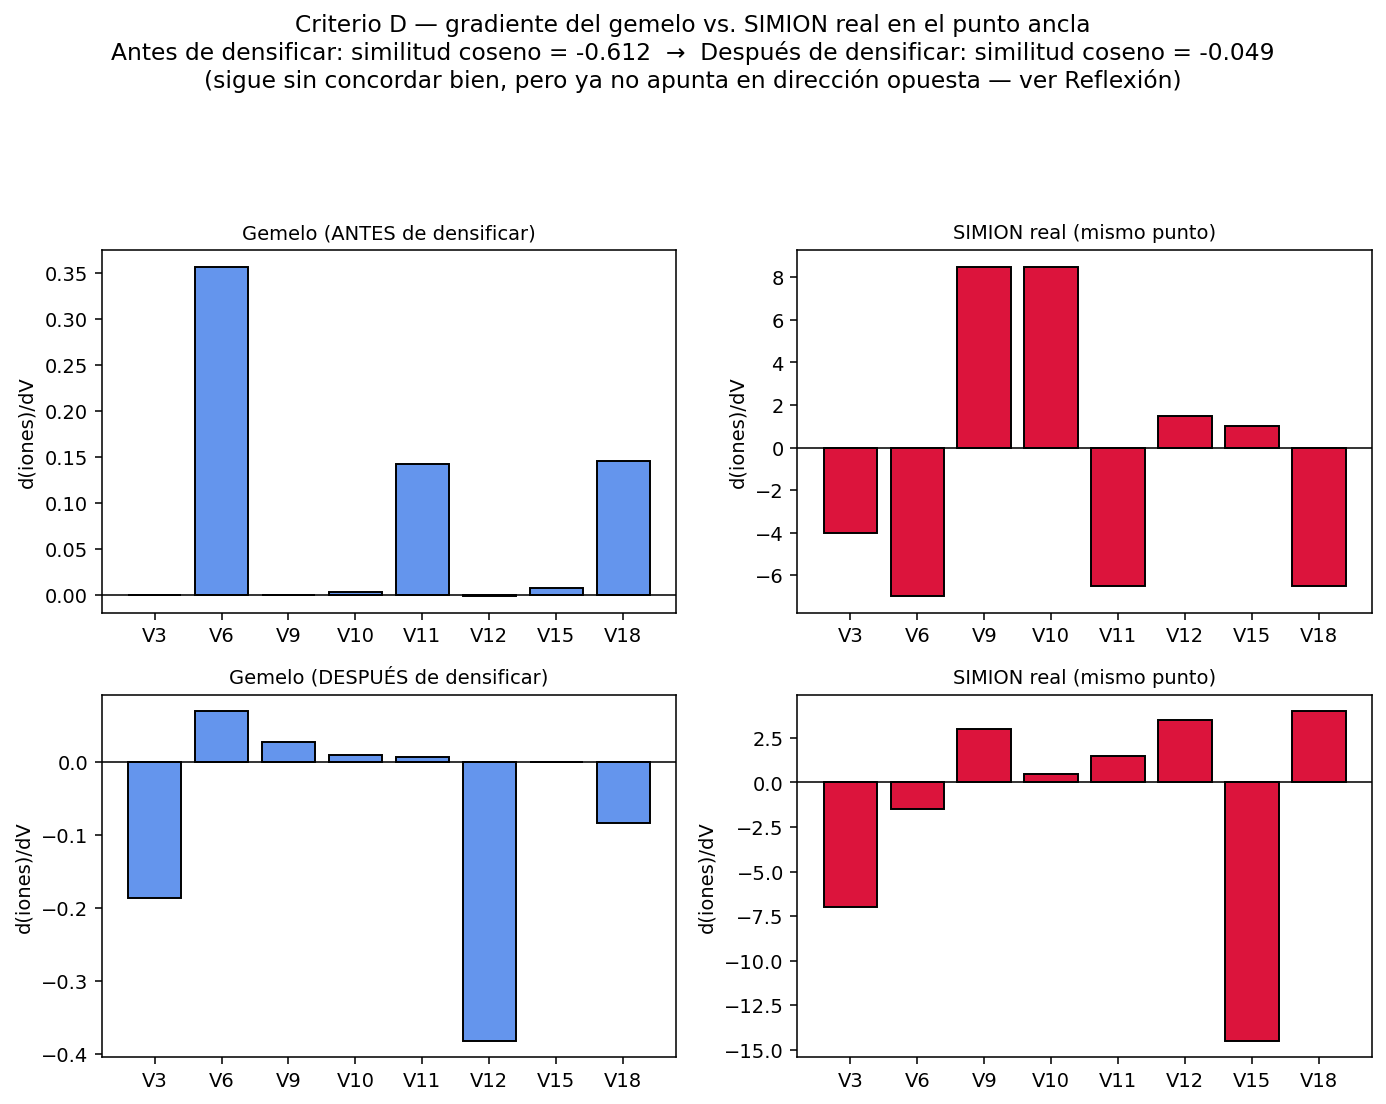
\includegraphics[width=0.85\textwidth]{figures/fig5_gradiente.png}
  \caption{Gradiente del gemelo vs.\ SIMION real, antes y después de la
  densificación local.}
  \label{fig:gradiente}
\end{figure}

\subsection{El paso $\varepsilon$ importa tanto como el modelo}

SIMION es ruidoso (Sección~\ref{sec:limitaciones}): incluso promediando 5
corridas, cada conteo conserva ${\sim}3$--$4$ iones de incertidumbre, y una
diferencia centrada con $\varepsilon=1\,$V hereda un ruido de
${\sim}2.8\,$iones/V -- mayor que el gradiente verdadero. El ``gradiente
real'' de referencia a $\varepsilon=1\,$V era, en buena parte, ruido puro.
Repitiendo el chequeo con pasos más grandes (16 puntos $\times$ 5 corridas
reales por cada $\varepsilon$, congelados en
\texttt{data/gradient\_eps\_study\_cache.npz}):

\begin{center}
\begin{tabular}{lccc}
\toprule
Paso $\varepsilon$ & 1\,V & 5\,V & 10\,V \\
\midrule
Similitud coseno & $-0.241$ & $\mathbf{+0.307}$ & $+0.059$ \\
\bottomrule
\end{tabular}
\end{center}

Con $\varepsilon=5\,$V la relación señal/ruido mejora y el gradiente del
gemelo \textbf{sí apunta en la dirección correcta}. Con $\varepsilon=10\,$V
vuelve a caer: el pico real tiene un ancho del orden de 10--20\,V, así que la
secante ya se sale de la campana (sesgo de curvatura). Existe una ventana
intermedia (${\sim}5\,$V) entre el ruido y el sesgo, y es ahí donde el
chequeo de diferenciabilidad es informativo (Figura~\ref{fig:gradiente_eps}).

\begin{figure}[H]
  \centering
  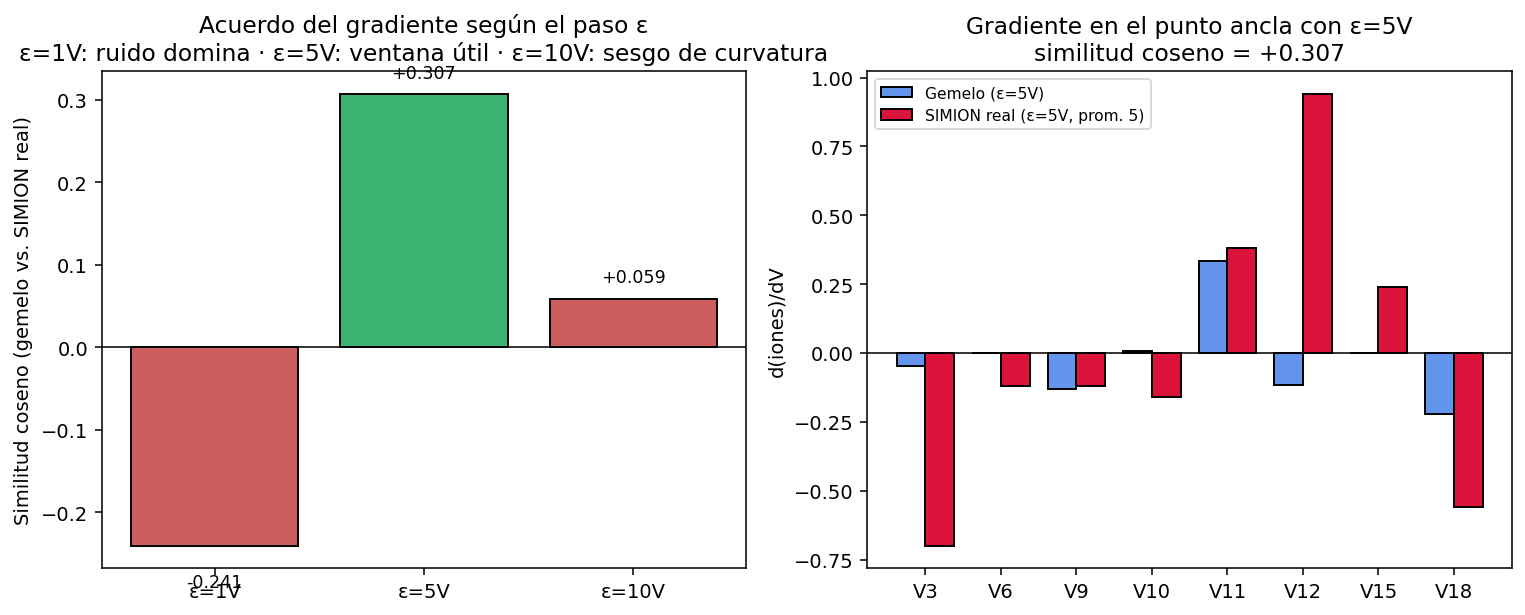
\includegraphics[width=0.95\textwidth]{figures/fig6_gradiente_eps.png}
  \caption{Izquierda: acuerdo del gradiente según el paso $\varepsilon$.
  Derecha: gradiente del gemelo vs.\ SIMION real con $\varepsilon=5$\,V,
  componente por componente.}
  \label{fig:gradiente_eps}
\end{figure}

Como chequeo adicional (\texttt{gradient\_retrain\_check.py}), reentrenar el
gemelo agregando las 16 sondas de $\varepsilon=10\,$V sube la similitud a
$+0.469$ contra el gradiente de $\varepsilon=5\,$V como conjunto
\emph{held-out} (evaluado sin usarlo en el entrenamiento, para no ser
circular). No se incorporó ese reentrenamiento al modelo entregado por la
misma razón de la Sección~\ref{sec:validacion-retrain}: mejora el gradiente
local a costa del ajuste global.

% =============================================================================
\section{Decisiones de diseño y alternativas descartadas}
% =============================================================================

\begin{itemize}
  \item \textbf{PINNs}: descartadas -- no hay una PDE simple que relacione 8
  voltajes con el conteo final; esa relación es la integración completa de
  trayectorias que SIMION ya resuelve.
  \item \textbf{GNN hamiltoniana}: descartada -- necesita datos de trayectoria
  que no se graban (\texttt{retain-trajectories=0}) y no hay estructura de
  grafo natural en 8 voltajes escalares.
  \item \textbf{Regresión simbólica}: se dejó como posible capa de
  interpretabilidad futura sobre el GP ya entrenado, no como modelo central
  (riesgosa en 8D con zona muerta).
  \item \textbf{GP simple, sin hurdle ni features físicas} (línea base):
  $R^2$ región informativa $=-0.338$, peor que predecir el promedio.
  Justificó el resto de las decisiones.
  \item \textbf{Hurdle model + features físicas}: subió el $R^2$ a $0.203$;
  cambiar el kernel a Matérn $\nu=1.5$ lo llevó a $0.237$.
  \item \textbf{Densificar con las 32 sondas de gradiente extra}: probado y
  descartado (Sección~\ref{sec:validacion-retrain}).
  \item \textbf{Optimización de control sin restricción}: falló
  catastróficamente (0 iones reales); el radio de confianza calibrado con
  SIMION real fue necesario.
\end{itemize}

% =============================================================================
\section{Limitaciones y trabajo futuro}
\label{sec:limitaciones}
% =============================================================================

\subsection{Ruido de SIMION}

El mismo punto exacto de voltajes da resultados distintos en corridas
separadas de SIMION (74, 60 y 63 iones observados para un mismo punto):
\texttt{SimpleSetUp.fly2} muestrea al azar la energía cinética y la dirección
de los 500 iones en cada vuelo, y \texttt{simion.seed()} solo puede invocarse
desde un programa Lua del workbench, no desde \texttt{--nogui fly}. La
mitigación adoptada en todo el proyecto es promediar 5 corridas reales para
cualquier número reportado como verificación
(\texttt{evaluate\_one\_real\_averaged}).

\subsection{Hasta dónde confiar en el gemelo}

El gemelo es confiable \textbf{dentro de vecindades de $\pm5\,$V de puntos
reales conocidos} (los resultados de control lo confirman); \textbf{no} para
optimización libre sobre todo el rango $\pm1000\,$V, donde puede estar
seguro y equivocado a la vez. El $R^2=0.237$ en la región informativa, aunque
mejor que la línea base, indica que el modelo no ha terminado de aprender la
forma fina del pico -- esperable con 45--61 puntos de señal en 8 dimensiones.

\subsection{Qué mejoraría con más presupuesto}

La mejora observada al pasar de 45 a 61 puntos de señal ($R^2$ de $0.056$ a
$0.203$, y a $0.237$ con el kernel final) sugiere que el techo aún no se
alcanza. Los puntos nuevos deberían repartirse (p.\ ej.\ con
\texttt{data\_collection.expandir\_activo()}, muestreo activo guiado por
incertidumbre) y no acumularse en el mismo sitio, ya que 32 sondas apiñadas
degradan el ajuste global (Sección~\ref{sec:validacion-retrain}). También
valdría la pena investigar la fuente residual de fallas de
\texttt{optimizer.py} (211 de 330 errores no se explican por la interferencia
de OneDrive confirmada).

% =============================================================================
\section{Conclusiones}
% =============================================================================

Con un presupuesto de 100 evaluaciones reales (más 16 de densificación local
dirigida), el gemelo digital:
\begin{itemize}
  \item predice la transmisión en la región informativa con $R^2=0.237$
  sobre 394 puntos de test reales nunca vistos;
  \item resuelve la tarea de dirección al 77\,\% del óptimo real conocido, y
  la consigna inversa con un error de 1.8 iones (menor que el ruido intrínseco
  de la máquina), siempre que la búsqueda se restrinja a una vecindad de
  confianza calibrada empíricamente con SIMION real;
  \item produce un gradiente que, medido a la escala de paso que el ruido de
  SIMION permite ($\varepsilon=5\,$V), concuerda en dirección con el
  gradiente real ($\cos=+0.307$).
\end{itemize}
El principal techo actual es la escasez de datos de señal en 8 dimensiones;
el camino más claro para mejorar el gemelo es más presupuesto de
entrenamiento repartido activamente cerca de la región de interés, no
simplemente más puntos en el mismo sitio.

\end{document}
